\documentclass[]{article}
\newcommand{\FileDepth}{../..}
\input{\FileDepth/Formats/AssignmentBasics.tex}
\usepackage{cancel}%This is special for Activities 4 and 5.
%opening
\newcommand{\SecType}{X}
\newcommand{\Week}{X}
\title{Two Blocks on a Frictionless Half-Ramp}
\author{Benjamin Bauml}
\date{Spring 2024}
\pagestyle{fancy}
\rhead{PH 221}
\chead{Spring 2024}
\lhead{Week \Week}

% For Assignment, leave Purpose as 1. For Worksheet, set to 2. For Student Solution, set to 3. For Teacher Solution, set to 4.
% If you want keep the pieces from being called manually, set DefOnly to 0.
\newcommand{\Purpose}{4}
\newcommand{\DefOnly}{1}

% Version 2024-04-27
% Changes
% 2024-02-21 Added xstring package to enable smooth implementation of new \ModePage command.
% 2024-04-27 Set up to split activities and formatting aspects into separate files. Removed dependence on xcomment. Added an automatic counter to number the activities in a problem set.
\usepackage{tcolorbox}
\usepackage{xstring}
% You will want the following four lines in your document (the last two uncommented):
% For Assignment, leave Purpose as 1. For Worksheet, set to 2. For Student Solution, set to 3. For Teacher Solution, set to 4.
% If you want keep the pieces from being called manually, set DefOnly to 0.
%\newcommand{\Purpose}{4}
%\newcommand{\DefOnly}{1}
\newcommand{\Exclusion}{0}
\newcommand{\PageTurn}{0}
\newcommand{\GrayProb}{0}
\newcommand{\Tipsy}{0}

% Assignment
\if\Purpose1
\renewcommand{\Exclusion}{1}
\fi
% Worksheet
\if\Purpose2
\renewcommand{\Exclusion}{1}
\renewcommand{\PageTurn}{1}
\fi
% Student Solution
\if\Purpose3
\renewcommand{\PageTurn}{1}
\renewcommand{\GrayProb}{1}
\fi
% Teaching Copy
\if\Purpose4
\renewcommand{\PageTurn}{1}
\renewcommand{\GrayProb}{1}
\renewcommand{\Tipsy}{1}
\fi

\def \NewQ {0}
\def \PForce {0}
\newcommand{\MaybePage}[1]{
	\def \PForce {#1}
	\if\PForce1
	\newpage
	\else
	\if\NewQ0
	\gdef \NewQ {\PageTurn}
	\else
	\newpage
	\fi
	\fi
}

\newcommand{\ModePage}[1]{
	\IfSubStr{#1}{\Purpose}{\newpage}{}
}

\newcounter{ActNumber}
\setcounter{ActNumber}{0}

\newcommand{\Problem}[4][0]{%The first argument is optional, and if it is set to 1, the \newpage will be forced. The second argument is the name of the activity, the third is the command the activity is stored as, and the fourth is the actual problem statement.
\newcommand{#3}{
\MaybePage{#1}
\addtocounter{ActNumber}{1}
\section*{\SecType\Week-\theActNumber: #2}
\if\GrayProb1
\begin{tcolorbox}[colback=lightgray,colframe=lightgray,sharp corners,boxsep=1pt,left=0pt,right=0pt,top=0pt,bottom=0pt,after skip=2pt]
\else
\begin{tcolorbox}[colback=white,colframe=white,sharp corners,boxsep=1pt,left=0pt,right=0pt,top=0pt,bottom=0pt,after skip=2pt]
\fi
#4
\end{tcolorbox}\noindent
}
\if\DefOnly0
\else
#3
\fi
}
	
\newcommand{\ProblemSub}[3][0]{%The first argument is optional, and if a string of numbers is entered into it, it will force a \newpage in any \Purpose that shows up in the string. For example, "13" would lead to the newpage being forced in modes 1 and 3. The second is the command the activity is stored as, and the third is the actual problem statement.
\newcommand{#2}{
\ModePage{#1}
\if\GrayProb1
\begin{tcolorbox}[colback=lightgray,colframe=lightgray,sharp corners,boxsep=1pt,left=0pt,right=0pt,top=0pt,bottom=0pt,after skip=2pt]
\else
\begin{tcolorbox}[colback=white,colframe=white,sharp corners,boxsep=1pt,left=0pt,right=0pt,top=0pt,bottom=0pt,after skip=2pt]
\fi
#3
\end{tcolorbox}\noindent
}
\if\DefOnly0
\else
#2
\fi
}
		
\newcommand{\Solution}[2]{%The first argument is the command the solution is stored as, and the second is the actual solution.
\newcommand{#1}{
\if\Exclusion0
#2
\fi
}
\if\DefOnly0
\else
#1
\fi
}
		
\newcommand{\ProblemFig}[2]{%The first argument is the command the figure is stored as, and the second is the actual figure.
\newcommand{#1}{
\begin{figure}[h]
#2
\end{figure}
}
\if\DefOnly0
\else
#1
\fi
}
		
\newcommand{\TeachingTips}[1]{
\if\Tipsy1
\begin{tcolorbox}[colback=lightgray,colframe=black]
#1
\end{tcolorbox}
\fi
}

\newcommand{\FBDaxes}[4][2]{
	\begin{scope}[shift={(#2)},rotate=#3]
		% x-axis
		\draw[thick,->] (-#1,0) -- (#1,0);
		\node[anchor=west] at (#1,0) {$x$};
		% y-axis
		\draw[thick,->] (0,-#1) -- (0,#1);
		\node[anchor=south] at (0,#1) {$y$};
		\coordinate (#4) at (0,0);
	\end{scope}
}
\newcommand{\FBDvectorMA}[4]{
	\begin{scope}[shift={(#1)}]
		\coordinate (#4tip) at ({#2*cos(#3)},{#2*sin(#3)});
		\draw[ultra thick,blue,->] (#1) -- (#4tip);
	\end{scope}
}
\newcommand{\FBDvectorXY}[3]{
	\begin{scope}[shift={(#1)}]
		\coordinate (#3tip) at (#2);
		\draw[ultra thick,blue,->] (0,0) -- (#3tip);
	\end{scope}
}
\newcommand{\FBDdot}[1]{
	\filldraw[black] (#1) circle (3pt);
}
\newcommand{\FBDbox}[5][1]{
	\begin{scope}[shift={(#2)},rotate=#3]
		\filldraw[color=black,fill=white,thick] ({-#1/2},{#1/2}) -- ({-#1/2},{-#1/2}) -- ({#1/2},{-#1/2}) -- ({#1/2},{#1/2}) -- cycle;
		% Left side coordinates
		\coordinate (#4ltq) at ({-#1/2},{#1/4});
		\coordinate (#4lcent) at ({-#1/2},0);
		\coordinate (#4lbq) at ({-#1/2},{-#1/4});
		% right side coordinates
		\coordinate (#4rtq) at ({#1/2},{#1/4});
		\coordinate (#4rcent) at ({#1/2},0);
		\coordinate (#4rbq) at ({#1/2},{-#1/4});
		% top coordinates
		\coordinate (#4tlq) at ({-#1/4},{#1/2});
		\coordinate (#4tcent) at (0,{#1/2});
		\coordinate (#4trq) at ({#1/4},{#1/2});
		% bottom coordinates
		\coordinate (#4blq) at ({-#1/4},{-#1/2});
		\coordinate (#4bcent) at (0,{-#1/2});
		\coordinate (#4brq) at ({#1/4},{-#1/2});
		% corners
		\coordinate (#4tl) at ({-#1/2},{#1/2});
		\coordinate (#4tr) at ({#1/2},{#1/2});
		\coordinate (#4bl) at ({-#1/2},{-#1/2});
		\coordinate (#4br) at ({#1/2},{-#1/2});
		\node at (0,0) {#5};
	\end{scope}
}

\begin{document}
\maketitle
\begin{center}
	This material is borrowed/adapted from Chapter 7 of the \textit{Student Workbook} for \textit{Physics for Scientists and Engineers}.
\end{center}

\Problem{Two Blocks on a Frictionless Half-Ramp}{\TBFricHRamp}{
Consider the situation depicted below. Friction is negligible for the blocks and surface, and we will assume the strings and pulley are ideal (massless, frictionless, etc.).
}
\ProblemFig{\TBFricHRampFig}{
\centering
\includegraphics[scale=1.2]{\FileDepth/Activities/Two_Blocks_on_a_Frictionless_Half-Ramp/Blocks_on_a_Half-Tilt_Frictionless}
}
\ProblemSub{\TBFricHRampA}{
(a) Draw a free-body diagram for each block.
}
\Solution{\TBFricHRampASol}{I will indicate the half-ramp with the subscript $R$ and the string with the subscript $S$.

\begin{figure}[h]
	\centering
	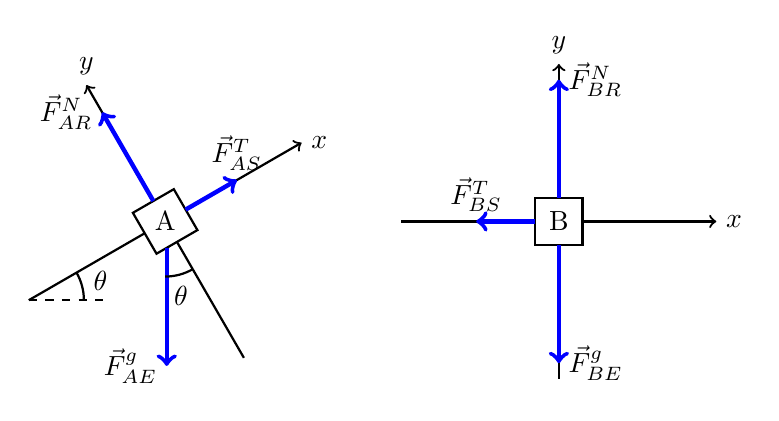
\begin{tikzpicture}
		\FBDaxes{-2.5,0}{30}{Aaxes}
		\FBDbox[0.6]{Aaxes}{30}{Abox}{A}
		\FBDvectorXY{Aboxblq}{0,-1.5}{FGA}
		\node[anchor=east] at (FGAtip) {$\vec{F}^{g}_{AE}$};
		\FBDvectorMA{Aboxrcent}{0.75}{30}{FTA}
		\node[anchor=south] at (FTAtip) {$\vec{F}^{T}_{AS}$};
		\FBDvectorMA{Aboxtcent}{1.3}{120}{FNA}
		\node[anchor=east] at (FNAtip) {$\vec{F}^{N}_{AR}$};
		\draw[thick] (-2.5,-0.7) arc (270:300:0.7);
		\node[anchor=north] at (-2.3,-0.7) {$\theta$};
		\begin{scope}[shift={(-2.5,0)}]
			\draw[thick,dashed] ({-2*cos(30)},-1) -- ({-2*cos(30)+1},-1);
			\draw[thick] ({-2*cos(30)+0.7},-1) arc (0:30:0.7);
			\node[anchor=south west] at ({-2*cos(30)+0.7},-1) {$\theta$};
		\end{scope}
		\FBDaxes{2.5,0}{0}{Baxes}
		\FBDbox[0.6]{Baxes}{0}{Bbox}{B}
		\FBDvectorXY{Bboxbcent}{0,-1.5}{FGB}
		\node[anchor=west] at (FGBtip) {$\vec{F}^{g}_{BE}$};
		\FBDvectorXY{Bboxtcent}{0,1.5}{FNB}
		\node[anchor=west] at (FNBtip) {$\vec{F}^{N}_{BR}$};
		\FBDvectorXY{Bboxlcent}{-0.75,0}{FTB}
		\node[anchor=south] at (FTBtip) {$\vec{F}^{T}_{BS}$};
	\end{tikzpicture}
\end{figure}
}
\TeachingTips{
This is one problem where it is imperative \underline{not} to use $G$ for ``ground'' to indicate the surface beneath the blocks. If you do, the force on block A by the ground will have a very unfortunate symbol: $\vec{F}_{AG}$. It may be rather uncomfortable to accidentally write something that looks like a slur in front of your students.
}
\ProblemSub{\TBFricHRampB}{
(b) Indicate the Newton’s third law pairs.
}
\Solution{\TBFricHRampBSol}{There are no third law pairs. $\vec{F}^{T}_{AS}$ and $\vec{F}^{T}_{BS}$ are equal in magnitude, but they are not opposite in direction, and they are not directly between boxes A and B, instead going through the string and pulley between them.

However, since these two forces are equal in magnitude (due to the ideality of the pulley and the string), I will simplify my notation by giving their magnitudes a single symbol: $F^{T} = F^{T}_{AS} = F^{T}_{BS}$.
}
\ProblemSub{\TBFricHRampC}{
(c) Find the normal force on each block.
}
\Solution{\TBFricHRampCSol}{In order to do this, I will write out Newton's second law in the $y$-direction for both blocks. Neither is accelerating perpendicular to the surface, so the net force in this direction is zero.
\begin{align*}
F^{net}_{A,y} & = F^{N}_{AR,y}+F^{g}_{AE,y} & F^{net}_{B,y} & = F^{N}_{BR,y}+F^{g}_{BE,y} \\
0 & = F^{N}_{AR}-m_{A}g\cos\theta & 0 & = F^{N}_{BR}-m_{B}g \\
F^{N}_{AR} & = m_{A}g\cos\theta & F^{N}_{BR} & = m_{B}g
\end{align*}
}
\ProblemSub{\TBFricHRampD}{
(d) Find the acceleration of the two blocks.
}
\Solution{\TBFricHRampDSol}{Both blocks accelerate in the $x$-direction, and since they are attached, they must have the same magnitude of acceleration. Also, since their coordinate systems agree on which direction along the surface is $+x$, the accelerations will also share the same sign. As such, I will use a single symbol for both accelerations: $a = a_{A,x} = a_{B,x}$.
\begin{align*}
	F^{net}_{A,x} & = F^{T}_{AS,x}+F^{g}_{AE,x} & F^{net}_{B,x} & = F^{T}_{BS,x} \\
	m_{A}a_{A,x} & = F^{T}-m_{A}g\sin\theta & m_{B}a_{B,x} & = -F^{T} \\
	m_{A}a & = F^{T}-m_{A}g\sin\theta & m_{B}a & = -F^{T}
\end{align*}
Adding these two equations together gives us
\begin{align*}
	(m_{A}+m_{B})a & = F^{T}-m_{A}g\sin\theta + (-F^{T}) = -m_{A}g\sin\theta \\
	a & = -\frac{m_{A}}{m_{A}+m_{B}}g\sin\theta
\end{align*}
The negative sign lets us know that these blocks will accelerate to the left.

In the special case where $m_{B} \ll m_{A}$, the fraction $\frac{m_{A}}{m_{A}+m_{B}}$ approaches 1, and we get $a = g\sin\theta$, which is the acceleration we expect from an object freely sliding down a ramp (which we expect to be the limiting case when there is no additional mass attached to A). Conversely, if $m_{B} \gg m_{A}$, then $\frac{m_{A}}{m_{A}+m_{B}} \approx \frac{m_{A}}{m_{B}} \approx 0$, and the blocks don't move. This we also expect, as a massive enough block B should not allow block A to move it, thus preventing any sliding.
}
\ProblemSub{\TBFricHRampE}{
(e) Find the tension in the string.
}
\Solution{\TBFricHRampESol}{We already know from part (d) that $F^{T} = -m_{B}a$, so we can substitute our answer for the acceleration into this to obtain
\[
F^{T} = \frac{m_{A}m_{B}}{m_{A}+m_{B}}g\sin\theta.
\]
If we wanted to do more algebra, we could also start with both equations from (d) and solve them for $F^{T}$ instead of for $a$:
\begin{align*}
	m_{A}a & = F^{T}-m_{A}g\sin\theta & m_{B}a & = -F^{T} \\
	m_{A}m_{B}a & = m_{B}F^{T}-m_{A}m_{B}g\sin\theta & m_{A}m_{B}a & = -m_{A}F^{T}
\end{align*}
Subtracting the right hand equation from the left hand equation gives us
\begin{align*}
	m_{A}m_{B}a - m_{A}m_{B}a & = m_{B}F^{T}-m_{A}m_{B}g\sin\theta - (-m_{A}F^{T}) \\
	0 & = (m_{A}+m_{B})F^{T} - m_{A}m_{B}g\sin\theta \\
	F^{T} & = \frac{m_{A}m_{B}}{m_{A}+m_{B}}g\sin\theta.
\end{align*}
Our answer is positive (for all sensible angles from 0$^{\circ}$ to 90$^{\circ}$), which should be the case for a magnitude of a vector. Sometimes, when we do force analysis and get a negative number, it just tells us that the direction we assumed for a force is backward from what it actually is, but in this case, getting a negative magnitude would tell us that something was wrong. After all, tension cannot push.

For $m_{A} \gg m_{B}$, we obtain $F^{T} \approx \frac{m_{A}m_{B}}{m_{A}}g\sin\theta = m_{B}g\sin\theta$. In this situation (as I mentioned in part (d)), block A is accelerating at $g\sin\theta$ down the ramp, so the force on block B needs to be just perfect to get it accelerating at $g\sin\theta$ to keep up.

Conversely, for $m_{B} \gg m_{A}$, we obtain $F^{T} \approx \frac{m_{A}m_{B}}{m_{B}}g\sin\theta = m_{A}g\sin\theta$. In this situation, both blocks are stationary (B is too massive to move), so the tension needs to be strong enough to counteract the $x$-component of the force of gravity on A and hold it in place.
}
\end{document}